\documentclass[pdftex,a4paper,12pt]{extarticle}
\usepackage[lmargin=1.25in,rmargin=1.25in,tmargin=1in,bmargin=1in]{geometry}
\usepackage[IL2]{fontenc}
\usepackage[T1]{fontenc}
\usepackage{lmodern}
\usepackage[utf8]{inputenc}
\usepackage[czech]{babel}
\usepackage[numbers]{natbib}
\usepackage{url}
\usepackage{booktabs}
\usepackage{amsmath}
\DeclareUrlCommand\url{\def\UrlLeft{<}\def\UrlRight{>} \urlstyle{tt}}
\usepackage{graphicx}
\usepackage{float}
\usepackage[usenames,dvipsnames]{xcolor}
\usepackage{listings}
\usepackage{needspace}
\usepackage{tikz}
\usepackage{array}



\usepackage{mathtools}
\usepackage[unicode,pdfdisplaydoctitle,pdftex,colorlinks,allcolors=black]{hyperref}
\hypersetup {pdftitle={KIV/VSS},pdfauthor={Kareš, Matěj; Kinkor, Vojtěch}}
\title{Vězňovo dilema s modelem důvěry}
\author{Matěj Kareš, Vojtěch Kinkor}
\date{\today}

\lstset{
	numbers=left,
	numberstyle=\ttfamily\fontfamily{pcr}\selectfont\color[HTML]{777777},
	frame=lines,
	framexleftmargin=0.5em,
	framexrightmargin=0.5em,
	xleftmargin=0.5em,
	xrightmargin=0.5em,
	rulecolor=\color[HTML]{555555},
	backgroundcolor=\color[HTML]{FCFCFC},
	showstringspaces=false,
	commentstyle=\itshape\color[HTML]{555555},
	keywordstyle=\color{blue},
	stringstyle=\color{ForestGreen},
	breakatwhitespace=true,
	breaklines=true,
	basicstyle=\footnotesize\ttfamily\fontfamily{pcr}\selectfont,
	keepspaces=true, 
	language=,
	tabsize=4,
	escapeinside={\%*}{*)},	 
	morekeywords={},
	postbreak=\raisebox{0ex}[0ex][0ex]{\ensuremath{\hookrightarrow\space}}
}

\newcommand*{\parvsp}{\par\vspace{\baselineskip}\noindent}
\renewcommand{\labelitemii}{$\circ$}
\mathcode`.="002C % replace dots in math mode with commas, https://www.fi.muni.cz/cstug/csfaq/sectT.html
\def\doteq{\buildrel\textstyle\ldotp\over=} % fix \doteq



\begin{document}

\hypersetup{pageanchor=false}
\begin{titlepage}
\begin{center}


~\\[1.5cm]

\includegraphics[width=0.6\textwidth]{res/logo}
\\[0.75cm]


{ \huge \bf Semestrální práce z předmětu\\ KIV/VSS \\[0.4cm] }
{ \LARGE \sc \begin{spacing}{0.9}Simulace hry \uv{vězňovo dilema}\end{spacing} }


\vfill

% Author and supervisor
\begin{minipage}[b]{0.49\textwidth}
\begin{flushleft} 
\emph{Datum:}\\[1mm]
\today
\end{flushleft}
\end{minipage}
\begin{minipage}[b]{0.49\textwidth}
\begin{flushright} 
\emph{Vypracovali:}\\[1mm]
Matěj \textsc{Kareš}\\ A16N0038P\\[1mm]
Vojtěch \textsc{Kinkor}\\ A16N0040P
\end{flushright}
\end{minipage}



\end{center}
\end{titlepage}
\hypersetup{pageanchor=true}

\newpage
\tableofcontents
\newpage

%ZADÁNÍ%
\section{Zadání}
\label{zadani}
Vytvořte simulátor pro úlohu z~teorie her -- iterované vězňovo dilema. Do simulace zakomponujte model důvěry, díky kterému lze simulovat např. chování různých etnických skupin vůči sobě. Práci vytvořte tak, aby bylo možné přidělávat nové vězně s~různými strategiemi a~parametry chování.

Simulace může mít jen textový výstup, grafický je vítaným rozšířením.

%TEORIE%
\newpage
\section{Teoretické pozadí}
\label{Teoretické pozadí}

\subsection{Vězňovo dilema}
\label{Vězňovo dilema}
Vězňovo dilema je v~teorii her úloha s~nenulovým součtem. Nechť jsou dva podezřelí posazeni do dvou různých místností a~vyšetřovatel se jich zeptá, jestli zločin, kvůli kterému jsou vyslýcháni, spáchal ten druhý. Vězni mají na výběr mlčet nebo vypovídat proti druhému. 

Jelikož máme dva vyslýchané, kteří mohou zvolit ze dvou možností, pak se výsledek výslechu může dostat do 4 stavů. 

\begin{enumerate}
\item \textbf{Spolupráce} je, když se oba vyslýchaní rozhodli mlčet a~jsou potrestání 1 rokem vězení oba.
\item \textbf{Nespolupráce} je, když se oba vyslýchaní rozhodli označit toho druhého jako viníka a~jsou oba potrestání 2 lety vězení oba.
\item \textbf{Podraz} nastává, kdy jeden vyslýchaný mlčí a~druhý vypovídá. V~této situaci je potrestán ten, kdo mlčel 3 lety, a~ten, který vypovídal, je propuštěn beztrestně.
\item Stejné jako bod 3, pouze první vypovídá a~druhý mlčí, tresty jsou stejné.
\end{enumerate}

Cílem každého vyslýchaného je mít co největší zisk (nejméně let ve vězení). Pokud sečteme roky strávené ve vězení u~jednotlivých výsledků výslechu, tak zjistíme, že spolupráce vede na dva roky ve vězení celkem, a~tak by bylo dobré vždy spolupracovat. Jenže pokud si myslíme, že bude ten druhý spolupracovat, je lepší ho podrazit, protože tím maximalizujeme osobní zisk (tedy 0 let). Pokud předpokládáme, že nás ten druhý podrazí, je opět lepší vypovídat proti němu, protože mlčení by nás poslalo do vězení na 3 roky, kdežto vypovídání v~tomto případě pouze na 2. V~posledním případě je opět vidět, že by pro komunitu bylo lepší aby jeden mlčel a~druhý vypovídal ($3 + 0 = 3$ roky vězení) než když vypovídají oba ($2 + 2 = 4$ roky vězení).

Právě tento konflikt osobního zisku a~zisku komunity dělá úlohu zajímavou, protože lze najít paralely v~reálném světě (marketing, mezinárodní vztahy, \dots).

\subsubsection{Strategie}
\label{Strategie}
Pro účely simulace existují základní strategie chování vyslýchaných. V~následujícím výčtu jsou uvedeny nepopulárnější.

\begin{description}
\item \textbf{Kavka} vždy spolupracuje.
\item \textbf{Podrazák} vždy podrazí.
\item \textbf{TFT} (Tit for tat) začíná spoluprací, pak už jen opakuje to, co udělal předchozí oponent. Pokud byl naposledy zrazen, zradí také, atd.
\item \textbf{TF2T} (Tit for 2 tats) zradí, až když byl dvakrát po sobě zrazen.
\item \textbf{Rozmar} se rozhoduje zcela náhodně.
\end{description}


\subsection{Model důvěry}
\label{Model důvěry}
Abychom lépe vysvětlili funkci modelu důvěry, je potřeba krátké seznámení s~celkovým kontextem. 

\begin{description}
\item \textbf{Osoba} je jedinec, který jen předvolán k~výslechu. Jedinci mají svoje strategie rozhodování.
\item \textbf{Etnikum} je skupina osob jedné národnosti, nebo skupina osob označená stejným jménem.
\item \textbf{Komunita} je množina všech etnik, tedy i množina všech osob.
\item \textbf{Bohatství/skóre} je vyčíslení fitness u~osob, etnik nebo komunity. Větší hodnota značí větší fitness. 
\end{description}

\textbf{Důvěra} je v~tomto případě procentuální vyjádření, jak jedna osoba věří druhé, nebo jak jedna osoba věří jinému etniku. Individuální důvěru značíme malým $t$, např. osoba Alice má vůči Bobovi hodnotu důvěry $t_{AB} = 1$, což znamená, že mu bezmezně věří. Bob má vůči Alici důvěru $t_{BA} = 0.6$ a~Alici spíše věří.

\textbf{Interakce} mezi osobami mohou změnit hodnotu důvěry. Například Alice i Bob si navzájem věří $t_{AB} = t_{BA} = 0.5$ a~při dalším výslechu se tedy rozhodují zcela nahodile. Alice se rozhodne spolupracovat ale Bob usoudí, že bude lepší podrazit Alici. Alice je tedy odsouzena na 3 roky a~tak rozhořčena sníží důvěru k~Bobovi na $t_{AB} = 0.4$. Bob zjistil, že Alice byla ochotna spolupracovat a~jelikož vzájemná spolupráce je výhodnější usoudí Bob, že příště bude Alici věřit a~bude také mlčet, čímž jeho hodnota důvěry vzroste na $t_{BA} = 0.4$ vůči Alici. Hodnoty změny důvěry lze samozřejmě upravovat dle potřeb simulace.

Posledním bodem modelu důvěry je \textbf{vliv příslušnosti k~etniku} na rozhodnutí u~výslechu. Nechť Alice je členkou skupiny červených a~Bob členem skupiny modrých. Jako v~předchozím příkladu si Alice i Bob navzájem věří ($t_{AB} = t_{BA} = 0.6$). Červení ale obecně spíše nevěří modrým (značíme velkým $T$) $T_{cm} = 0.4$. Modří bezmezně věří červeným ($T_{mc} = 1$). Rozhodnutí vypočteme následovně:

$$R_A = t_{AB} \cdot 2T_{cm} = 0.6 \cdot 2 \cdot 0.4 = 0.48$$

Alice bude na 48 \% spolupracovat.

$$R_B = t_{BA} \cdot 2T_{mc} = 0.6 \cdot 2 \cdot 1 = 1.2$$

Bob bude na 100 \% spolupracovat (hodnoty nad 100 \% se ořezávají)


\subsection{Simulace rasismu}
\label{Simulace rasismu}
Zajímavou oblastí této úlohy je vytvoření různých skupin, které budou mít vzájemně různé hodnoty důvěry. O~tomto jsme se letmo zmínili v~části \ref{Model důvěry}. Rasismus spočívá v~předpojatosti vůči některé rase. Přestože mohu mít dobrý počáteční stav s~každým, vezmu v~potaz názor \uv{mé rasy} vůči ostatním, což ovlivní moje finální rozhodnutí. 

Stejně jako u~individuálních důvěr mohu dát své rase zpětnou vazbu o~tom, jak dopadl můj poslední soud, a~zvýšit tak důvěru celé rasy.


%ŘEŠENÍ%
\newpage
\section{Řešení úlohy}
\label{Řešení úlohy}

\subsection{Standardní algoritmy s modelem důvěry}
\label{Standardní algoritmy s modelem důvěry}
V~části \ref{Vězňovo dilema} jsme popsali některé základní algoritmy pro provádění simulace. Tyto algoritmy neuvažují model důvěry a~je potřeba je modifikovat. 

U~osob a~etnik lze nastavit jejich počáteční důvěru, o~kolik se má zvyšovat v~případě oponentovy spolupráce a~o~kolik se má snižovat v~případě oponentovy zrady. Tyto tři parametry budeme dále uvádět jako vektor tří čísel např. $\mathbf{[0.5; 0.1; 0.05]}$. Nyní můžeme popsat standardní algoritmy vektorem důvěry $\vec{t}$, aby splňovali jejich původní znění. Je nutné brát v~potaz, že velkou roli u~modelu důvěry hraje náhoda, a~proto uvažujeme počet iterací jdoucí do nekonečna. 

\begin{description}
\item \textbf{Kavka} $\mathbf{[1; 0; 0]}$ všem na začátku věří, výsledky soudu nijak nemění důvěru. 
\item \textbf{Podrazák} $\mathbf{[0; 0; 0]}$ nikomu na začátku nevěří, výsledky soudu nijak nemění důvěru.
\item \textbf{TFT} $\mathbf{[1; 1; 1]}$ začíná spoluprací, protože věří všem. Je-li s~ním spolupracováno důvěřuje i nadále. Je-li zrazen ztrácí veškerou důvěru dokud s~ním není opět spolupracováno.
\item \textbf{TF2T} $\mathbf{[1; 1; 0.5]}$ začíná spoluprací. Je-li zrazen, sníží svou důvěru na polovinu, je-li zrazen podruhé, sníží svoji důvěru na 0. Každá spolupráce vrátí důvěru zpět na 1. Tento algoritmus se při rozhodování s určitým stupněm náhody nebude chovat přesně jako bez modelu důvěry, protože existuje šance, že podrazí už po prvním podrazu. Je tedy lepší používat verzi bez modelu důvěry, záleží-li nám na přesném chování.
\item \textbf{Rozmar} $\mathbf{[0.5; 0; 0]}$ rozhoduje se nahodile, výsledky soudů ho neovlivňují. 
\end{description}


Další persony si může programátor přidělat sám dle připravených abstraktních tříd. Je nutno podotknout, že model důvěry lze ve vlastních personách ignorovat a~vytvářet tak strategie rozhodování, které důvěru neberou v~potaz. 

%PROGRAMÁTORSKÁ PŘÍRUČKA%
\newpage
\section{Programátorská příručka}
\label{Programátorská příručka}
Výsledná aplikace je implementována v jazyce Java 1.8. Pro překompilování aplikace lze použít nástroj Maven s přiloženým souborem \texttt{pom.xml}.

Pro vytváření vlastních person slouží abstraktní třída \texttt{SuspectedPerson}. Po zdědění je nutno implementovat metodu \texttt{public boolean decide(Person opponent)}, kde získáte referenci na oponenta (tedy toho, s~kým je persona u~výslechu). Strategie rozhodování je čistě na vašem uvážení. Metoda vrací \texttt{true} (spolupracovat) nebo \texttt{false} (podrazit). 

Třída \texttt{Game} obstarává průběh simulace. Vybírá osoby k~výslechu, spravuje komunitu a~s~pomocí třídy \texttt{GameHistory} zaznamenává proběhlé operace, soudy, bohatství a~úrovně důvěry.

Třídy \texttt{Kavka}, \texttt{Podrazak}, \texttt{TitForTat}, \texttt{TitForTwoTats} a~\texttt{Rozmar} jsou standardní algoritmy popsané v~\ref{Strategie} a~k~nim byla dále vytvořena třída \texttt{Optimalni}, která zná všechny předchozí strategie a~umí vhodně zvolit svoje akce aby maximalizovala zisk komunity. Tyto třídy lze použít jako inspiraci pro psaní vlastních tříd.

Třída \texttt{TrustRobotPerson} spolupracuje pouze pokud je důvěra k~oponentovi větší nebo rovna $0.5$, v opačném případě podráží. Jedná se o~velmi jednoduché znázornění jak se používá individuální důvěra pro rozhodování bez dalších vlivů (např. náhody).

Třída \texttt{TrustComplexPerson} zohledňuje individuální důvěru a~důvěru etnických skupin. Jedná se o~znázornění využití celého modelu důvěry. V~této třídě lze také vidět, jak se modifikují individuální i skupinové důvěry na základě výsledku z~předchozího soudu. Tato třída by měla být výchozím bodem pro další persony a~na programátorovi je jen upravit si parametry rozhodování, případně napsat vlastní algoritmus rozhodování.

%UŽIVATELSKÁ PŘÍRUČKA%
\newpage
\section{Uživatelská příručka}
\label{Uživatelská příručka}

\subsection{Spuštění programu}
\label{Spuštění}
Program lze spustit zadáním příkazu:\footnote{Předpokládá se spouštění na PC s~nainstalovaným JRE.}

\vspace{2mm}
\texttt{> java -jar PrisonersDilemma.jar}
\vspace{2mm}

Po spuštění proběhne simulace podle scénáře, který je součástí zdrojového kódu\footnote{Při vývoji nových algoritmů se předpokládá editace tohoto scénáře.}. Výstupem programu jsou statistiky vypsané na standardní výstup (skóre celé komunity, skóre jednotlivých etnik a~vývoj během simulace -- skóre a~důvěra jednotlivých etnik). Dále je zobrazen graf vývoje v~samostatném GUI okně.

\parvsp
Program je možné spustit s~vlastními scénáři pomocí parametru, např.:

\vspace{2mm}
\texttt{> java -jar PrisonersDilemma.jar script.basic.js}
\vspace{2mm}

V~tomto případě se scénář simulace načítá ze souboru \texttt{script.basic.js}. Jedná se o~skripty v~jazyce JavaScript, které je možné měnit bez překompilování aplikace. 

\parvsp
Součástí práce jsou tři předpřipravené skripty:

\begin{description}

\item \texttt{script.basic.js} provede simulaci pomocí základních strategií (\texttt{Kavka}, \texttt{Podrazak}, \texttt{TFT}, \texttt{TF2T}, \texttt{Rozmar}, \texttt{Optimalni}; každá persona je v~komunitě obsažena právě jednou)

\item \texttt{script.tft-robots.js} obsahuje simulaci dvou person \texttt{TrustRobotPerson} s~parametry $\mathbf{[0.0; 1.0; 1.0]}$, resp. $\mathbf{[1.0; 1.0; 1.0]}$. Simulují tedy chování algoritmu TFT, přičemž od prvního kola kola hrají opačně a~zisk celé společnosti zůstává nulový.

\item \texttt{script.trust.js} obsahuje simulaci dvou person \texttt{TrustComplexPerson} zařazených do dvou etnik, Red a~Blue. Na počátku je důvěra Blue vůči Red úplná ($t_{Blue\to Red}=1$) a~Red vůči Blue nulová ($t_{Red\to Blue}=0$). Persony se dále liší v~rychlosti růstu důvěry vůči druhému. Výchozí důvěra vůči jedinci je neutrální ($0.5$). Simulace ve většině případů skončí ve stavu, kdy i Red začne Blue věřit a~oba jedinci začnou spolupracovat. Vlivem náhodného rozhodování při částečné důvěře ale může nastat opačná situace, tedy že Blue začne podrážet a~důvěra obou etnik i jedinců postupně klesne na nulu.

\end{description}

Syntaxe skriptů je popsána v~jednotlivých souborech pomocí komentářů.

%VÝSLEDKY%
\newpage
\section{Výsledky}
\label{Výsledky}

Spuštění programu bez parametru proběhne podle předdefinovaného scénáře. Vizualizaci je možné vidět na obrázku \ref{fig:chart1}. 

\begin{figure}[h]
  \centering
    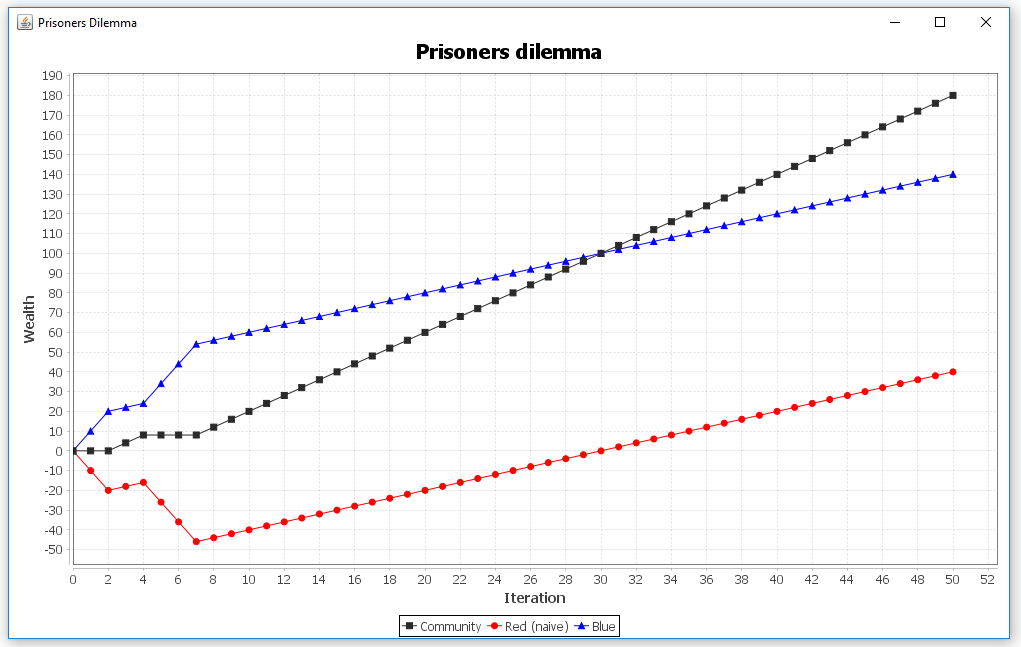
\includegraphics[width=\textwidth]{res/chart1.png}
    \caption{Vizualizace po spuštění bez parametru}
    \label{fig:chart1}
\end{figure}

Na obrázku \ref{fig:chart1} je červeně naznačen naivní algoritmus (spolupracující) a~modře je naznačen algoritmus který druhému nevěří. Do 7. iterace se bohatství červeného propadá, protože se snaží spolupracovat ale modrý ho neustále podráží. Později však červený ztratil v~modrého důvěru natolik, že se rozhodl také podrážet.    

\begin{figure}[h]
  \centering
    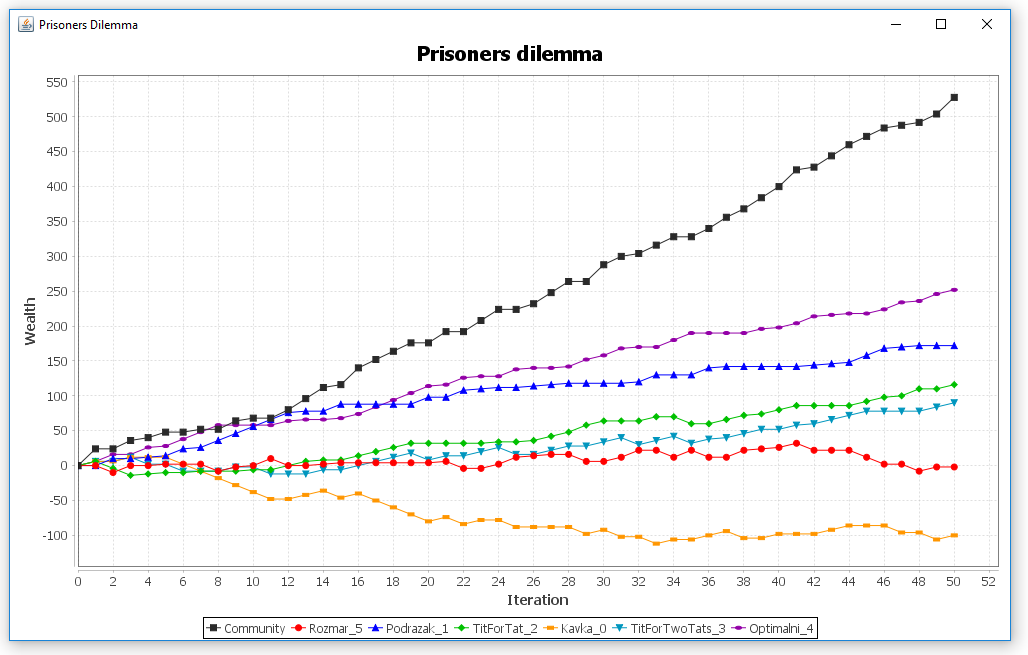
\includegraphics[width=\textwidth]{res/chart2.png}
    \caption{Vizualizace po spuštění bez parametru}
    \label{fig:chart2}
    \vspace{10mm}
\end{figure}

Na obrázku \ref{fig:chart2} je vidět porovnání všech základních algoritmů. Je patrné, že podrážet ve všech případech je nejvýhodnější cesta, protože nese nejméně rizik. Není zdaleka tak lukrativní, jako v~případě všech spolupracujících. Pokud však známe soupeře, a~víme jak se rozhodne, můžeme učinit informované rozhodnutí a~vydělat více na spolupracích, proto optimální algoritmus skutečně dostává svému jménu.

Důležitou poznámkou je, že výsledky mohou být pro stejná data jiné, protože vybírání párů k~výslechu je náhodné. Vybírání dvojic lze programově nastavit, aby bylo více deterministické.

%ZÁVĚR%
\newpage
\section{Závěr}
\label{Závěr}

Zadání bylo splněno v~celém rozsahu. Podařilo se nám vytvořit simulátor pro vězňovo dilema. Aplikace je vytvořena tak, aby v~ní mohli uživatelé vytvářet vlastní scénáře, vlastní komunity a~díky modelu důvěry také zkoušet vliv předpojatosti a~rasismu. Během návrhu byl kladen důraz na pozdější rozšíření a~bylo tak umožněno dědění obecných tříd, aby si uživatel mohl definovat vlastní persony, etnika, strategie a~předpojatosti dle svých potřeb. Restrikce při tvorbě vlastních prvků byly sníženy a~je tedy vyžadována určitá znalost domény pro používání.

Součástí práce je jednoduchá vizualizace simulovaného světa, kde si uživatel může prohlídnout vývoj společnosti pro jím zvolenou konfiguraci komunity. Výstup je grafický i textový. 

\end{document} 


